\documentclass{beamer}
\usepackage{listings}
\lstset{
%language=C,
frame=single,
breaklines=true,
columns=fullflexible
}
\usepackage{subcaption}
\usepackage{url}
\usepackage{tikz}
\usepackage{tkz-euclide} % loads  TikZ and tkz-base
%\usetkzobj{all}
\usetikzlibrary{calc,math}
\usetikzlibrary{shapes.geometric, arrows}
\usepackage{float}
\newcommand\norm[1]{\left\lVert#1\right\rVert}
\newcommand{\myvec}[1]{\ensuremath{\begin{pmatrix}#1\end{pmatrix}}}
\newcommand{\sgn}{\mathop{\mathrm{sgn}}}
\renewcommand{\vec}[1]{\mathbf{#1}}
\usepackage[export]{adjustbox}
\usepackage[utf8]{inputenc}
\usepackage{amsmath}
\usetheme{Boadilla}

\DeclareMathOperator{\sinc}{sinc}
\DeclareMathOperator{\rect}{rect}

\title{GATE EC-2018 Q39}
\author{Perambuduri Srikaran}
\institute{IITH AI}
%\date{}
\begin{document}
\providecommand{\pr}[1]{\ensuremath{\Pr\left(#1\right)}}
\providecommand{\qfunc}[1]{\ensuremath{Q\left(#1\right)}}
\providecommand{\sbrak}[1]{\ensuremath{{}\left[#1\right]}}
\providecommand{\lsbrak}[1]{\ensuremath{{}\left[#1\right.}}
\providecommand{\rsbrak}[1]{\ensuremath{{}\left.#1\right]}}
\providecommand{\brak}[1]{\ensuremath{\left(#1\right)}}
\providecommand{\lbrak}[1]{\ensuremath{\left(#1\right.}}
\providecommand{\rbrak}[1]{\ensuremath{\left.#1\right)}}
\providecommand{\cbrak}[1]{\ensuremath{\left\{#1\right\}}}
\providecommand{\lcbrak}[1]{\ensuremath{\left\{#1\right.}}
\providecommand{\rcbrak}[1]{\ensuremath{\left.#1\right\}}}
\providecommand{\fourier}{\overset{\mathcal{F}}{ \rightleftharpoons}}

\begin{frame}
\titlepage
\end{frame}
\section{Question}
\begin{frame}
\frametitle{Question}
\begin{block}{}
The input $4\sinc{\brak{2t}}$ is fed to a Hilbert transformer to obtain $y\brak{t}$, as shown in the figure below:
\tikzstyle{noborder} = [rectangle, draw=none, fill=white!50,
    text centered, rounded corners, minimum height=2em]
\tikzstyle{block} = [rectangle, draw, fill=white!50,
    text width=4.5em, text centered, minimum height=2em]
\tikzstyle{line} = [draw, -latex']
\begin{center}
\begin{tikzpicture}
[node distance = 2.8cm, auto]
    \node [noborder, fill opacity = 0, text opacity = 1] (init){$4\sinc{\brak{2t}}$};
    \node [block, right of = init, fill opacity = 0, text opacity = 1] (transformer){Hilbert Transform};
    \node [noborder, right of = transformer, fill opacity = 0, text opacity = 1] (result){$y\brak{t}$};

     \path [line] (init) -- (transformer);
     \path [line] (transformer) -- (result);
\end{tikzpicture}
\end{center}
Here, $\sinc{\brak{x}} = \frac{\sin\brak{\pi x}}{\pi x}$. The value (accurate to two decimal places) of $\int_{-\infty}^{\infty} |y\brak{t}|^2 dt$ is
\end{block}
\end{frame}
\section*{Solution}
\begin{frame}[fragile]
\frametitle{Parseval's Theorem}
\begin{flushleft}
Parseval's theorem states that there is no loss of information in Fourier transform and the amount of energy remains the same in time and frequency domains.
\begin{align}
    \int_{-\infty}^{\infty} |x\brak{t}|^{2} dt = \int_{-\infty}^{\infty} |X\brak{f}|^{2} df
\end{align}
\end{flushleft}
\end{frame}
\begin{frame}[fragile]
\frametitle{Solution}
\begin{flushleft}
We will define the following functions:
\begin{align}
    x(t) &= 4\sinc(2t)\\
    h(t) &= \frac{1}{\pi t}\\
    y(t) &= x(t) * h(t) \label{eq:1}\\
    x(t) &\fourier{X(f)}\\
    h(t) &\fourier{H(f)}\\
    y(t) &\fourier{Y(f)}
\end{align}
\end{flushleft}
\end{frame}
\begin{frame}[fragile]
\frametitle{Solution Contd...}
\begin{flushleft}
Define the rectangular function,
\begin{align}
    \rect(t) =
    \begin{cases}
    1 & \text{if } |t| \leq \frac{1}{2}\\
    0 & \text{if } |t| > \frac{1}{2}
    \end{cases}
\end{align}
Define the signum function,
\begin{align}
    \sgn(t) =
    \begin{cases}
    1 & \text{if } t > 0\\
    0 & \text{if } t = 0\\
    -1 & \text{if } t < 0
    \end{cases}
\end{align}
\end{flushleft}
\end{frame}
\begin{frame}[fragile]
\frametitle{Solution Contd...}
\begin{flushleft}
The Fourier transforms are
\begin{align}
    X(f) &= 2\rect\brak{\frac{f}{2}}\\
    H(f) &= -j\sgn(f)
\end{align}
Applying Convolution theorem in \eqref{eq:1},
\begin{align}
    Y(f) &= X(f)H(f)\\
    &= -2j\rect\brak{\frac{f}{2}}\sgn(f)\\
    &= 2j\rect\brak{f + \frac{1}{2}} - 2j\rect\brak{f - \frac{1}{2}}
\end{align}
\end{flushleft}
\end{frame}
\begin{frame}[fragile]
\frametitle{Solution Contd...}
\begin{flushleft}
Applying Inverse Fourier Transform on $Y(f)$,
\begin{align}
    y(t) &= 2j\sinc(t)e^{-j\pi t} - 2j\sinc(t)e^{j\pi t}\\
    &= -2j\sinc(t)\brak{e^{j\pi t} - e^{-j\pi t}}\\
    &= 2\sinc(t)\brak{\frac{e^{j\pi t} - e^{-j\pi t}}{j}}\\
    &= 4\sinc(t)\sin(\pi t)\\
    &= 4\pi t\sinc^2(t)
\end{align}
\end{flushleft}
\end{frame}
\begin{frame}[fragile]
\frametitle{Solution Contd...}
\begin{flushleft}
By the Parseval's theorem,
\begin{align}
    \int_{-\infty}^{\infty} |y\brak{t}|^{2} dt &= \int_{-\infty}^{\infty} |Y\brak{f}|^{2} df\\
    &= \int_{-1}^{1} |2\rect(f)|^2df\\
    &= 8
\end{align}
\end{flushleft}
\end{frame}
\begin{frame}[fragile]
\frametitle{Plots}
\begin{columns}
\begin{column}{0.5\textwidth}
\begin{figure}[htp]
\begin{flushleft}
    \centering
    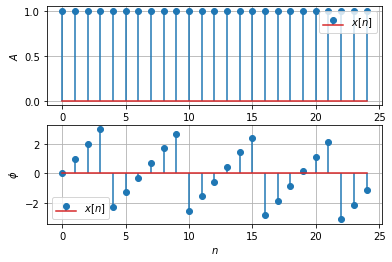
\includegraphics[width=\columnwidth]{Fig1.png}
    \caption{Input and Output Signals}
    \label{fig:plot1}
\end{flushleft}
\end{figure}
\end{column}
\begin{column}{0.5\textwidth}
\begin{figure}[htp]
\begin{flushleft}
    \centering
    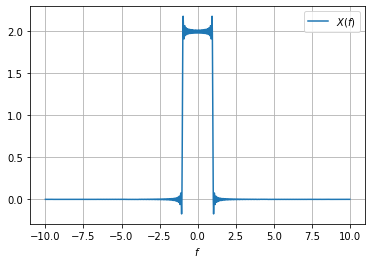
\includegraphics[width=\columnwidth]{Fig5.png}
    \caption{Plots of X(f) in frequency domain}
    \label{fig:plot1}
\end{flushleft}
\end{figure}
\end{column}
\end{columns}
\end{frame}
\begin{frame}[fragile]
\frametitle{Plots}
\begin{columns}
\begin{column}{0.5\textwidth}
\begin{figure}[htp]
\begin{flushleft}
    \centering
    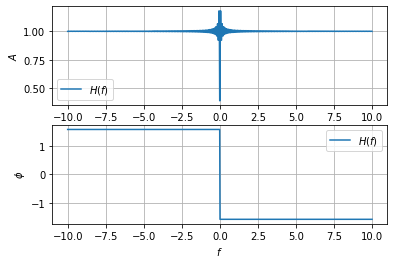
\includegraphics[width=\columnwidth]{Fig4.png}
    \caption{Amplitude and Phase of H(f) v/s frequency}
    \label{fig:plot1}
\end{flushleft}
\end{figure}
\end{column}
\begin{column}{0.5\textwidth}
\begin{figure}[htp]
\begin{flushleft}
    \centering
    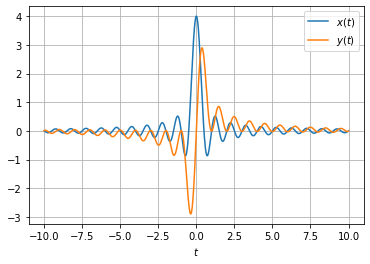
\includegraphics[width=\columnwidth]{Fig2.png}
    \caption{Amplitude and Phase of Y(f) v/s frequency}
    \label{fig:plot1}
\end{flushleft}
\end{figure}
\end{column}
\end{columns}
\end{frame}
\end{document}
